% =====================================================================
%  MoRE -- LIGHT 2026 (NeurIPS workshop) long-paper submission
%
%  BUILD:  pdflatex main -> bibtex main -> pdflatex main -> pdflatex main
%
%  MODE:   bare \usepackage{neurips_2026} == SUBMISSION mode.
%          Authors are replaced by "Anonymous Author(s)" and lineno is on.
%          For camera-ready switch to [dblblindworkshop, final] and add
%          \workshoptitle{...} (mandatory with the workshop options).
%
%  NEVER edit neurips_2026.sty. Geometry changes are grounds for desk
%  rejection, and the style file floors \tiny/\scriptsize/\footnotesize
%  at 6/7/8 pt so shrinking a table past that is not available anyway.
%
%  PAGE BUDGET: 9 content pages (LIGHT CFP, long-paper track); references,
%  appendices, acknowledgments and the checklist do NOT count. Target 8.0.
%
%  FIGURES: every figure is a compiling PLACEHOLDER box. To drop in the
%  real artwork, comment out \figplaceholder and uncomment the
%  \includegraphics line directly beneath it. Nothing else changes.
% =====================================================================
\documentclass{article}

\usepackage{neurips_2026}

% -- template's own shell list --
\usepackage[utf8]{inputenc}
\usepackage[T1]{fontenc}
\usepackage{hyperref}
\usepackage{url}
\usepackage{booktabs}
\usepackage{amsfonts}
\usepackage{nicefrac}
\usepackage{microtype}
\usepackage{xcolor}
\usepackage{graphicx}
\usepackage{subcaption}
\providecommand{\justification}[1]{#1}

% -- ADDED: the shell omits all three, and each is load-bearing 
% amsmath MUST be loaded before \begin{document} or neurips_2026.sty
% cannot patch equation/align for lineno, and reviewer line numbers in
% the margin silently go wrong.
\usepackage{amsmath}
\usepackage{graphicx}     % the shell loads NO graphics package
\usepackage{subcaption}   % two-panel Figure 2
\usepackage{enumitem}     % compact lists; the shell has no list control

% -- figure placeholder 
\newcommand{\figplaceholder}[2]{%
  \setlength{\fboxsep}{0pt}%
  \fbox{\parbox[c][#2][c]{\dimexpr\linewidth-2\fboxrule\relax}{%
    \centering\footnotesize\ttfamily [PLACEHOLDER]\\[2pt]#1}}%
}

\title{Mixture of Recursive Experts: Does Mixing Sparse Expert
Routing with Adaptive Recursion Pay Off?}

% In submission mode this block is ignored and replaced by
% "Anonymous Author(s)". Fill it in for camera-ready.
\author{%
  Anonymous \\
  Affiliation \\
  \texttt{email} \\
}

\begin{document}

\maketitle

\begin{abstract}
Sparse routing decides \emph{which} token an expert receives;
adaptive recursion decides \emph{how much}. Both are sold as ways to spend
less compute per token, and the two mechanisms are orthogonal in principle,
so composing them is an obvious thing to try. We try it. Mixture of Recursive
Experts (MoRE) routes each token to one of six independent expert FFNs and
then reuses that expert's weights for an adaptive number of recursion steps
under Adaptive Computation Time halting. Measured against routing alone and
recursion alone at a matched budget of 3.2\,M parameters, on a synthetic
arithmetic-reasoning benchmark with known routing and depth ground truth, the
composition does not pay off. Recursion alone is lowest-loss; MoRE is
statistically indistinguishable from routing alone while running
$3.81\times$ slower, on a sixth of the FFN arithmetic. The halting policy is
mechanically adaptive, with gradients reaching the halt head and 99.97\% of
tokens exiting early, but it is not behaviorally adaptive: a constant-depth
policy that ignores its input beats both learned halt heads on 5 of 5 seeds,
and forcing every token to maximum depth fits better than learning when to
stop.
\end{abstract}

\section{Introduction}

Conditional computation comes in two flavors that answer different questions.
Sparse mixture-of-experts layers \citep{jacobs1991moe,shazeer2017moe,
fedus2022switch} answer \emph{which computation module should process this
token}, dispatching each token to a small number of independent
sub-networks. Recursive weight-tied architectures with learned halting
\citep{graves2016act,dehghani2019ut,banino2021pondernet} answer \emph{how much
computation does this token need}, reusing one block for a variable number of
steps. Both are motivated by the same accounting argument: most tokens do not
need the full model, so spend less on them.

The two mechanisms are orthogonal, which makes their composition an obvious
candidate. Route a token to a specialized expert, then let that expert's
weights be reused for as many steps as the token appears to need. The resulting
architecture: MoRE which inherits an efficiency argument from each side. What
it does not inherit is evidence: whether the composition beats either component
at a matched budget has not, to our knowledge, been isolated yet.

We tried to isolate it. One training engine implements three configurations differing
only in the fields their definitions require: routing without recursion (MoE,
six experts, depth 1), recursion without routing (MoR, one shared block, depth
up to 7), and the composition (MoRE, six experts, depth up to 7). All three sit
at $\approx$3.2\,M parameters, share a bit-identical input representation, and
train on the same fixed split of a synthetic arithmetic benchmark in which the
correct expert and the intended recursion depth of every token are known by
construction.

Four results follow: MoR reaches the
lowest validation loss; MoRE is indistinguishable from MoE
($p = 0.6587$); the learned halt heads lose to the best input-independent
constant depth on every seed of both recursive arms; and forcing maximum depth
improves loss at unchanged throughput. We report this as a negative result
about the composition at this scale, not as a claim about either mechanism in
general.

\textbf{Contributions.}
\begin{itemize}[leftmargin=1.4em,itemsep=1pt,topsep=2pt]
\item An exactly parameter-matched isolation of adaptive recursion. MoE
  \emph{is} MoRE at \texttt{max\_depth}~$=1$: identical tensor shapes,
  identical 3{,}201{,}555 parameters, one field changed. The MoRE-vs-MoE
  contrast therefore varies recursion and nothing else.
\item A benchmark, \texttt{more6-v1}, with per-token routing ground truth and
  a per-operation target-depth curriculum, plus a machine-checked input
  contract: permuting the oracle expert index changes zero input features.
\item A constant-depth null model, which we argue is the minimum bar any
  adaptive-depth claim must clear, and the finding that neither halt head
  clears it.
\item A six-arm ablation with family-wise error control, which separates
  routing quality from predictive quality. Supervising the router to perfect
  routing accuracy makes the task loss worse.
\end{itemize}

This is an exploratory paper on the architecture, aimed to check if its viable in the very least.

\section{Related Work}

\textbf{Sparse expert routing.} Conditional mixtures of local experts date
to \citet{jacobs1991moe}; the sparsely-gated form that made them practical at
scale is due to \citet{shazeer2017moe}, with Top-1 dispatch, load-balancing
auxiliaries and the capacity-factor machinery developed in GShard
\citep{lepikhin2021gshard}, Switch Transformer \citep{fedus2022switch} and
ST-MoE \citep{zoph2022stmoe}. The standard justification is parameters at
constant FLOPs. That argument is unavailable here by construction: we pin all
three arms to the same parameter count, so what remains of the sparsity case
is a wall-clock case, which \S\ref{sec:cost} tests directly.

\textbf{Adaptive depth and weight-tied recursion.} Adaptive Computation
Time \citep{graves2016act} introduced the learned per-step halting unit we
use; Universal Transformers \citep{dehghani2019ut} applied it to a weight-tied
transformer block, and PonderNet \citep{banino2021pondernet} reformulated the
halting distribution to improve its gradient. Early-exit variants place the
decision at the layer or token level instead \citep{elbayad2020depthadaptive,
schuster2022calm,raposo2024mod}. Weight tying itself is well established as a
parameter-reduction device \citep{lan2020albert}. What this literature reports
is overwhelmingly \emph{mean} step counts and exit-rate histograms. We argue
in \S\ref{sec:depth} that neither statistic tests input-dependence, and that
the comparison which does  against the best constant policy  is rarely
made.

\textbf{Composing the two.} Recent work has begun to combine routing with
recursion, most directly by using a router to assign per-token recursion
depth \citep{bae2025mor,raposo2024mod}. Those systems route \emph{to depths}
over shared weights. MoRE differs in that routing selects among genuinely
independent expert FFNs and the recursion then reuses \emph{that expert's}
weights, so the two decisions are made by different heads over different
objects. We are not aware of a matched-budget comparison of such a composition
against each of its components, which is the gap this paper fills. We make no
novelty claim for the combination itself.

\section{Mixture of Recursive Experts}
\label{sec:more}

\subsection{Problem setting and notation}

A record is a program of $S \le 7$ arithmetic steps. Step $s$ carries a
numeric argument vector $\mathbf{a}_s \in \mathbb{R}^{12}$ and an operation
identifier $o_s$ drawn from 16 integer operations. The model reads the
sequence of steps and regresses the final scalar answer $y$. Write $E$ for
the number of experts, $T$ for the maximum recursion depth, $d$ for the model
width, and $\mathbf{h}^{(0)}_s \in \mathbb{R}^{d}$ for the input embedding of
step $s$, formed by projecting $\mathbf{a}_s$ and adding a learned embedding
of $o_s$.

Two things are deliberately absent from $\mathbf{h}^{(0)}_s$. The step's
\emph{result} is excluded, because for the final step it is the regression
target. The oracle expert index is excluded, because supplying it would make
the routing problem trivial; operation identity enters instead as an
embedding, which is legitimate task information. \S\ref{sec:data} reports the
machine check that both exclusions hold.

\subsection{The MoRE block}

Routing happens once per token (Figure~\ref{fig:architecture}). A linear router
produces
$\mathbf{g} = \mathrm{softmax}(W_r \mathbf{h}^{(0)}_s) \in \Delta^{E-1}$, the
token is assigned to $e^\star = \arg\max_e g_e$, and \emph{only} that expert
is evaluated:
\begin{equation}
\mathbf{h}^{(t+1)} \;=\; \mathrm{LayerNorm}\!\left(
  \mathbf{h}^{(t)} + g_{e^\star}\cdot \mathrm{FFN}_{e^\star}\!\left(\mathbf{h}^{(t)}\right)
\right), \qquad t = 0,\dots,T-1 .
\label{eq:block}
\end{equation}
The gate probability $g_{e^\star}$ multiplies the expert output, which is what
carries task-loss gradient into the router: the discrete $\arg\max$ is not
differentiated, but the scalar that scales the selected expert's contribution
is. The expert index is fixed for the token, so the recursion in
Eq.~\ref{eq:block} reuses the \emph{same} expert parameters at every depth.
There is one block ($\mathrm{FFN}_{e}$ is not indexed by $t$), so depth is
computation through time rather than a stack of depth-specific layers, and no
capacity limit is imposed: every routed token is evaluated by its expert and
none is dropped.

\begin{figure}[t]
    \centering
    \includegraphics[width=11cm,keepaspectratio]{fig/More(3).png}
    \caption{The MoRE block. A token is routed once to one of $E$ independent
    expert FFNs; that expert's weights are then reused for an adaptive number of
    recursion steps under ACT halting. Setting $T=1$ recovers MoE exactly and
    setting $E=1$ recovers MoR; the input representation is bit-identical in all
    three cases.}
    \label{fig:architecture}
\end{figure}

\subsection{Halting and the training objective}

Halting follows ACT \citep{graves2016act} with one halt head per expert. At
each step the selected expert's head emits
$p_t = \sigma(\mathbf{w}_{e^\star}^{\!\top}\mathbf{h}^{(t)})$, cumulative mass
$c_t = \sum_{\tau \le t} p_\tau$ accumulates, and the token halts as soon as
$c_t + p_t > 1 - \epsilon$ with $\epsilon = 0.01$, receiving remainder
$R = 1 - c_t$ as its final weight. Tokens still active at $t = T$ are forced
out. Halted states are frozen and not recomputed, so a halted token costs
nothing at deeper steps. The boolean comparison decides dispatch only; the
differentiable path to the halt parameters runs through the expected depth
\begin{equation}
\rho \;=\; \mathbb{E}_{\text{tokens}}\big[\,N + R\,\big],
\label{eq:ponder}
\end{equation}
in which the step count $N$ is discrete and contributes no gradient while the
remainder $R$ does. Eq.~\ref{eq:ponder} is the ponder cost.

The training objective is a weighted sum of terms that we report separately
and never as a single number:
\begin{equation}
\mathcal{L} \;=\;
\underbrace{\mathcal{L}_{\text{task}}}_{1.0} \;+\;
\underbrace{0.5\,\mathcal{L}_{\text{fam}}}_{\text{external labels}} \;+\;
0.001\,\mathcal{L}_{\text{bal}} \;+\;
0.001\,\rho \;+\;
\underbrace{0.0 \cdot \mathcal{L}_{\text{route}}}_{\text{off}} .
\label{eq:loss}
\end{equation}
$\mathcal{L}_{\text{task}}$ is mean squared error on the normalized final
answer. $\mathcal{L}_{\text{bal}} = -H(\bar{\mathbf{g}}) + E\sum_e f_e
\bar{g}_e$ combines a router-entropy bonus with the Switch-style auxiliary
\citep{fedus2022switch}, where $f_e$ is the dispatched load fraction and
$\bar{\mathbf{g}}$ the mean soft router probability; it is averaged over the
depth calls actually made, so its magnitude does not grow with $T$. Weighted, it
is $1.3\%$ of the task term, a diagnostic not an objective.
$\mathcal{L}_{\text{route}}$ is a routing-supervision term against the oracle
expert index, carried at weight zero in the canonical configuration so its
magnitude stays visible while contributing no gradient; \S\ref{sec:abl} reports
what happens when it is switched on. One disclosure belongs with
Eq.~\ref{eq:loss}: $\mathcal{L}_{\text{fam}}$ is a whole-program family
cross-entropy trained on labels read off disk, so it is external annotation
rather than self-supervision, and at weight $0.5$ it is the second-largest term.
The canonical router is therefore not entirely unsupervised in the loose sense,
even though the per-token routing decision receives no oracle signal.

\subsection{One engine, three modes}
\label{sec:engine}

MoE, MoR and MoRE are configurations of one implementation with an explicit
\texttt{architecture} mode, not three codebases. They share one data
pipeline, one optimizer setup and one evaluation path, so a difference between
them cannot be a difference in the harness. Only the fields their definitions
require differ: $E \in \{6,1,6\}$, $T \in \{1,7,7\}$, MoR's FFN multiplier
(below), and the two loss weights for quantities that do not exist in a given
arm (no ponder cost at depth 1, nothing to balance with one expert).

We write \textbf{MoR} for our recursion-only configuration  one shared
block with adaptive halting  which is in the spirit of weight-tied
recursive transformers with learned halting
\citep{dehghani2019ut,bae2025mor} but is not a reproduction of any specific
published system; all three arms are configurations of the same engine.

\textbf{Matching the budget.} MoR has one FFN where MoRE has six, so
matching the per-FFN multiplier would compare 3.2\,M parameters against
0.57\,M and call the difference architectural. We instead equalize
\emph{total} FFN hidden width, giving MoR's single FFN a multiplier of
$24 = 4 \times 6$. All three arms then hold exactly 3{,}145{,}728 FFN
weight-matrix parameters. MoE and MoRE are parameter-\emph{identical} at
3{,}201{,}555; MoR sits $0.12\%$ lower at 3{,}197{,}710, the residual being
six per-expert halt heads, the router and FFN biases. That residual is
irreducible at any integer multiplier, and it runs \emph{against} our headline
result: the arm with slightly fewer parameters is the one that wins.

\section{Experimental setup}\label{sec:setup}

\subsection{The \texttt{more6-v1} benchmark}
\label{sec:data}

\texttt{more6-v1} contains 70,000 synthetic integer-arithmetic programs generated by a seeded script. Sixteen operations form six families: \textsc{add/sub}, \textsc{mult/div}, \textsc{mod/pow}, \textsc{logic}, \textsc{shift}, \textsc{sort/stat} which provide routing ground truth. About 40\% of records are multi-operation chains; since MoRE routes per token, their steps route individually to the six families, and the record lacks a whole-program family label (masked, not a seventh class). Discarding these would remove all programs of length 4--7, making depth allocation unmeasurable. Splits are fixed files of 59,500 / 5,250 / 5,250 with zero program-key overlap across splits and no duplicates within splits; seed-to-seed variance arises only from initialization, dropout, and batch order.

The depth curriculum assigns target depths per operation: 1 for \textsc{add}/\textsc{sub}/\textsc{logic}/\textsc{shift}, 2 for \textsc{mult}/\textsc{div}/\textsc{max}/\textsc{min}, 3 for \textsc{mod}/\textsc{pow}, and 4 for \textsc{median}/\textsc{sort}. This is independent of expert index: \textsc{logic} and \textsc{shift} both target 1, while \textsc{sort/stat} spans 2 and 4. Thus, scoring well on depth cannot rely on routing alone, making \S\ref{sec:depth} independent of \S\ref{sec:routing}. The curriculum is hand-authored and treated as a design assumption rather than absolute correctness.

An automated audit confirms the input contract: step results and oracle expert indices are absent from features, and feature ranges are identical across arms. On the normalized target, predicting the training mean yields MSE 0.080914, while copying the best single input feature yields 0.081853, so no copy strategy is competitive; all $R^2$ values are relative to the 0.080914 floor. Appendix~\ref{app:detail} provides the full audit.

\subsection{Protocol and metrics}\label{sec:protocol}
\label{sec:protocol}

Every canonical arm is run at seeds $\{42,43,44,45,46\}$ and reported as
mean\,$\pm$\,std over five runs. Training is 50 epochs of AdamW
($\text{lr}=10^{-3}$, weight decay $10^{-4}$) with cosine annealing, batch
768, gradient clipping at 1.0, dropout 0.1, $d = 256$, $T = 7$, on one RTX
4060 Laptop GPU (8\,GB). These optimizer settings were fixed once, before the
comparison, and \emph{not} swept per architecture; we report them as a stable
operating point rather than as a tuned optimum, and no arm was tuned for
itself.

The primary metric is validation task loss at the \emph{final} epoch. We
deliberately do not select on best-epoch validation loss: that is an order
statistic whose downward bias scales with each arm's per-epoch validation
noise, which is not matched across architectures. Best-epoch values are
reported as a secondary column so the selection effect stays checkable.

Comparisons use an exact two-sided randomization test on the difference of
means, and every $p$ is accompanied by the smallest value the arm sizes can
produce, $p_{\min} = 1/\binom{n_a+n_b}{n_a}$: $0.0040$ at five-versus-five and
$0.0179$ at three-versus-five. A $p$ at its floor is the test's resolution
limit, not a strong result. We do not use the phrase ``statistically
significant'' anywhere; differences are described as resolvable or not
resolvable at five seeds, with the $p$-value quoted.

Because the router is unsupervised, expert indices carry no semantic identity,
so raw routing accuracy measures label permutation as much as partition quality.
We report it once and then rely on Hungarian-matched accuracy, adjusted mutual
information \citep{vinh2010ami} and cluster purity. Entropy is reported
normalized as $H/\log E$ and treated strictly as a load-balance diagnostic. For
depth we report mean steps, absolute and relative \emph{depth allocation error}
against the curriculum, and exit rates; depth is measured offline in eval mode
on the held-out split (Appendix~\ref{app:caveats}).

\section{Results}

\subsection{Predictive quality}
\label{sec:quality}

Table~\ref{tab:main} is the headline. Recursion alone is lowest-loss. MoR
beats MoE by $0.000554$ ($d = 4.13$, $p = 0.0079$) and beats MoRE by
$0.000481$ ($d = 2.49$, $p = 0.0159$). MoRE and MoE are not distinguishable at
five seeds: the gap is $-0.000074$ in MoRE's favor with $p = 0.6587$, and
since MoE \emph{is} MoRE with $T$ set to 1 and the same 3{,}201{,}555
parameters, this is an exact isolation of recursion. Adding adaptive recursion
on top of expert routing changed nothing measurable. Adding expert routing on
top of recursion made things worse.

\begin{table}[t]
\centering
\footnotesize
\caption{Canonical results, 5 seeds each, mean\,$\pm$\,std. Primary metric is
final-epoch validation task loss; \emph{best-ep.} is the minimum over
evaluated epochs, shown only so the selection effect stays visible. $R^2$ is
against the predict-train-mean floor of $0.080914$. Routing columns are
\textsc{n/a} for MoR because one expert admits no partition  not $0$; their
seed standard deviations are $0.056/0.085/0.063$ (MoE) and $0.061/0.074/0.062$
(MoRE), omitted from the cells for width.
Pairwise, on the primary metric: MoE${-}$MoR $+0.000554$ ($d\,4.13$,
$p\,0.0079$); MoRE${-}$MoR $+0.000481$ ($d\,2.49$, $p\,0.0159$);
MoRE${-}$MoE $-0.000074$ ($d\,{-}0.36$, $p\,0.6587$). Exact two-sided
randomization test, $p_{\min} = 0.0040$. Throughput is this implementation on
one laptop GPU (\S\ref{sec:cost}).}
\label{tab:main}
\vspace{2pt}
\begin{tabular}{lrlrrrrrr}
\toprule
& Params & val task loss & $R^2$ & best-ep. & tok/s & Hung. & AMI & Purity \\
\midrule
MoE  & 3{,}201{,}555 & 0.063260\,$\pm$\,0.000153 & 0.2182 & 0.062819 & 8485 & 0.500 & \textbf{0.513} & 0.572 \\
MoR  & 3{,}197{,}710 & \textbf{0.062706\,$\pm$\,0.000112} & \textbf{0.2250} & 0.062527 & 4574 & \textsc{n/a} & \textsc{n/a} & \textsc{n/a} \\
MoRE & 3{,}201{,}555 & 0.063186\,$\pm$\,0.000249 & 0.2191 & 0.062892 & 2225 & \textbf{0.526} & 0.491 & \textbf{0.605} \\
\bottomrule
\end{tabular}
\end{table}

One thing bounds how much weight this ordering carries. The best $R^2$ is
$0.2250$: all three arms explain roughly a fifth of target variance, and the
entire between-architecture spread is about $3\%$ of what they explain, so the
task representation rather than the architecture is the binding constraint here, 
\S\ref{sec:abl} reaches the same conclusion from the capacity side. The
models are nonetheless clearly learning: every arm beats the constant-mean
floor, the best single-feature copy and the zero predictor.

The training side reverses the ordering. MoRE reaches the \emph{lowest} training
loss of the three ($0.060237 \pm 0.000360$ against MoE's $0.060453$ and MoR's
$0.061501$), so its validation deficit is not a failure to fit. Generalization
gaps are $0.002949$ (MoRE), $0.002807$ (MoE) and $0.001205$ (MoR) 
$2.4\times$ smaller for the single-expert arm. The ordering tracks expert count,
not depth: MoE has no recursion and essentially MoRE's gap. A coherent reading is
that each of six experts sees roughly a sixth of the data, which affords more
room to memorize per unit of shared weight than the whole of it does; we offer
that as a reading, not a finding, since settling it needs a width or
dataset-size sweep we did not run.

\subsection{Is the halting policy input-dependent?}
\label{sec:depth}

The halting mechanism functions as intended: gradients reach the halt heads, tokens exit early almost always ($99.86\%$ for MoR, $99.97\%$ for MoRE), and forced exits at $T=7$ are rare ($0.14\%$ and $0.03\%$). The learned mean step count of $2.13$ closely matches the benchmark's token-weighted target depth of $2.11$. Reported as mean and exit histogram, the policy appears successful.

However, the mean alone cannot determine if token depth depends on the token itself. To test this, we assign every token the same depth $c$, ignoring its operation, sweeping $c$ over $[0.5,7.0]$ in steps of $0.01$ on 19,843 held-out tokens. The best constant is $c=2.00$, outperforming both learned policies (Table~\ref{tab:depth}, Figure~\ref{fig:depth}). MoR's mean absolute depth error is $8.3\%$ worse than the constant; MoRE's is $14.2\%$ worse, consistent across all seeds and pooled ($p=0.00195$ under a sign test).

One objection is that learned policies' means differ from 2, so deficits might stem from worse means rather than allocation. Evaluating constants at each arm's mean, the constant scores $0.9127$ at $c=2.13$ versus MoR's $0.9423$, and $0.9844$ at $c=2.35$ versus MoRE's $0.9940$. Thus, deficits arise from allocation, not averages.

Histograms (Figure~\ref{fig:depth-hist}) show MoR places $97.1 \pm 1.1\%$ of tokens at exactly two steps; MoRE places $92.7 \pm 3.2\%$ at two and $4.9 \pm 3.8\%$ at three. Both converge near a constant, and the small variation does not align with token complexity. Because absolute error is convex in predicted depth, uncorrelated variation is penalized relative to the best constant, explaining observed deficits. This excludes aligned variation but cannot distinguish misaligned signal from noise.

MoRE is mechanically more adaptive but less accurate: it runs $0.2248$ steps deeper ($d=2.88$, $p=0.0079$), carries more halting remainder ($0.2651$ vs. $0.1283$), and incurs $9.3\%$ higher ponder cost, yet its absolute depth error is $0.0517$ higher ($p=0.3571$) and relative error $0.0995$ higher ($p=0.0159$). Conditioning the halt head on routed experts increased dispersion without improving alignment.

% The halting mechanism works in the sense that it is asked to: gradients reach
% the halt heads, tokens exit early almost always ($99.86\%$ for MoR, $99.97\%$
% for MoRE), forced exits at $T = 7$ are rare ($0.14\%$ and $0.03\%$), and the
% learned mean step count of $2.13$ lands close to the benchmark's
% token-weighted target depth of $2.11$. Reported the way this literature
% usually reports it  a mean and an exit histogram  the policy looks
% successful.

% It is not. The question a mean cannot answer is whether the depth a token
% receives depends on \emph{that token}. We answer it with the cheapest possible
% competitor: give every token the same depth $c$, ignore its operation
% entirely, and sweep $c$ over $[0.5, 7.0]$ in steps of $0.01$ on the same
% 19{,}843 held-out step-tokens. The best constant is $c = 2.00$, and it beats
% both learned policies (Table~\ref{tab:depth}, Figure~\ref{fig:depth}). MoR's
% mean absolute depth error
% is $8.3\%$ worse than a constant; MoRE's is $14.2\%$ worse. This holds in
% $5/5$ seeds per arm and $10/10$ pooled, so under a sign test the pooled
% $p = 0.00195$; per arm the test floors at $p = 0.0625$ at $n = 5$, which is
% why we pool.

\begin{table}[t]
\centering
\footnotesize
\caption{Depth allocation on the held-out split, measured offline from each
run's best-validation checkpoint, 5 seeds. Errors are per-token
$|{\hat{d}} - d^\star|$ against the benchmark's per-operation target depth.
The third row is not a model: it assigns every token the same depth, swept to
its optimum. Deltas are against that row. The target depth distribution over
these tokens is $38.1\%/28.2\%/18.5\%/15.2\%$ at depths $1/2/3/4$, so a
constant of 2 is wrong by at least one step on $71.8\%$ of them and still
wins.}
\label{tab:depth}
\vspace{2pt}
\begin{tabular}{llllll}
\toprule
& mean steps & abs.\ depth err. & $\Delta$ & rel.\ err. & early exit \\
\midrule
MoR  & 2.1283\,$\pm$\,0.0188 & 0.9423\,$\pm$\,0.0266 & $+0.0720$ & 0.5939\,$\pm$\,0.0225 & 0.9986 \\
MoRE & 2.3531\,$\pm$\,0.1087 & 0.9940\,$\pm$\,0.1054 & $+0.1237$ & 0.6934\,$\pm$\,0.0931 & 0.9997 \\
\midrule
constant $c = 2.00$ & 2.0000 & \textbf{0.8703} &  & \textbf{0.5186} &  \\
\bottomrule
\end{tabular}
\end{table}

% One objection has to be closed off: the learned policies do not average exactly
% 2, so their deficit could come from a worse mean rather than worse allocation.
% Reading the sweep at each arm's own mean, the constant scores $0.9127$ at
% $c = 2.13$ against MoR's $0.9423$, and $0.9844$ at $c = 2.35$ against MoRE's
% $0.9940$. The deficit is in the allocation, not the average.

% The histograms in Figure~\ref{fig:depth-hist} say why. MoR places
% $97.1 \pm 1.1\%$ of tokens at exactly two steps; MoRE places $92.7 \pm 3.2\%$
% at two and $4.9 \pm 3.8\%$ at three. Both have converged to within a few percent
% of a constant, and the few percent that vary do not vary in the right direction.
% Because absolute error is convex in the predicted depth, variation uncorrelated
% with the target is penalized relative to the best constant, which is what we
% observe; this rules out variation \emph{aligned} with token complexity but does
% not separate misaligned signal from noise.

% MoRE is the more adaptive of the two by every mechanical measure and the worse
% by every accuracy measure. It runs $0.2248$ steps deeper ($d = 2.88$,
% $p = 0.0079$), carries more halting remainder ($0.2651$ vs $0.1283$) and pays
% $9.3\%$ more ponder cost, yet its absolute depth error is $0.0517$ higher
% ($p = 0.3571$) and its relative error $0.0995$ higher ($p = 0.0159$).
% Conditioning the halt head on the routed expert bought dispersion without
% buying alignment.

\begin{figure}[t]
    \centering

    \begin{subfigure}[t]{0.48\linewidth}
        \centering
        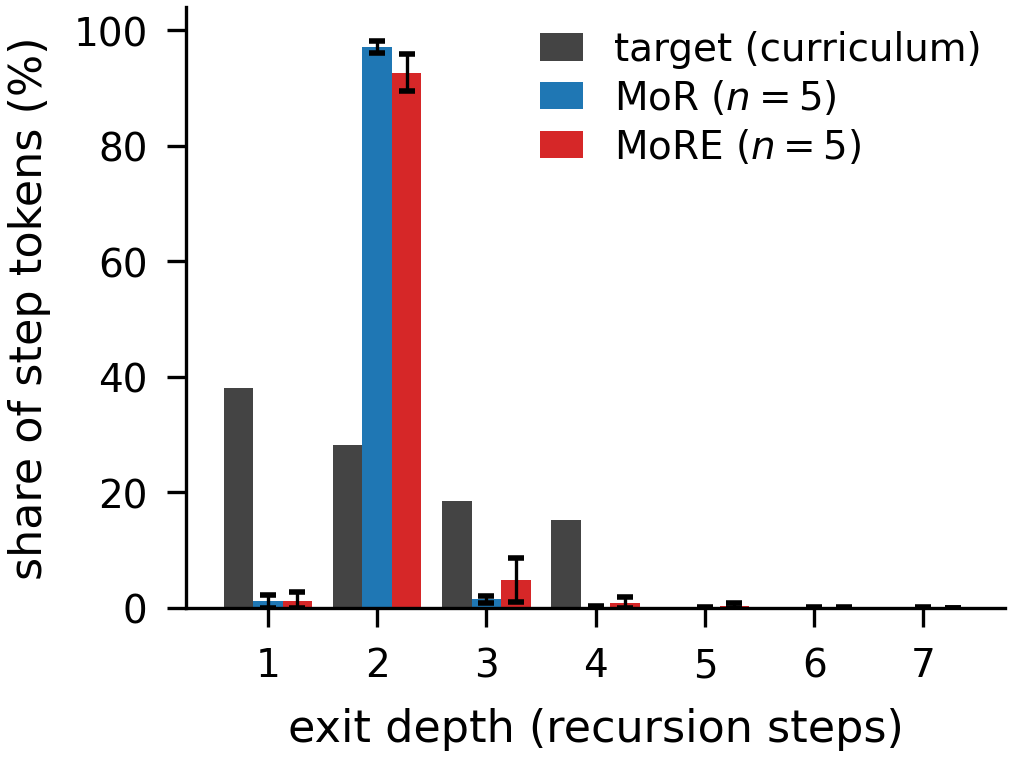
\includegraphics[width=4.5cm,keepaspectratio]{fig/fig2a_depth_hist.png}
        \caption{Predicted vs target depth.}
        \label{fig:depth-hist}
    \end{subfigure}
    \hfill
    \begin{subfigure}[t]{0.48\linewidth}
        \centering
        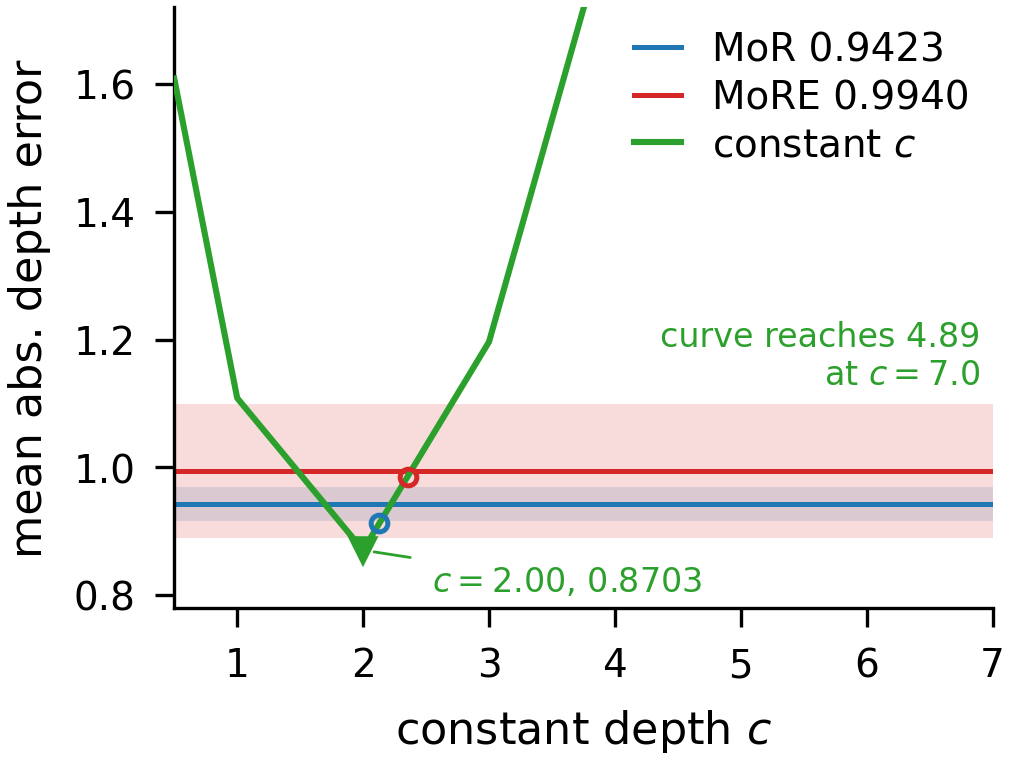
\includegraphics[width=4.5cm,keepaspectratio]{fig/fig2b_depth_null.png}
        \caption{Learned policies vs the best constant.}
        \label{fig:depth-null}
    \end{subfigure}

    \vspace{0.5em}

    \caption{Adaptive depth is mechanically active and behaviorally near-constant.
    Left: both learned policies collapse most of their mass onto two steps while
    the target spreads over four. Right: no learned policy reaches the constant
    baseline's error, at its own mean or anywhere else.}
    \label{fig:depth}
\end{figure}

\subsection{Expert specialization}
\label{sec:routing}

Expert indices carry no semantic identity, so raw agreement with the oracle
family is close to meaningless: it is $0.2016 \pm 0.1578$ for MoE and
$0.1629 \pm 0.1864$ for MoRE, both with a standard deviation larger than the
distance from chance ($1/6 = 0.1667$), because each seed permutes the labels
differently. Every claim below therefore rests on permutation-invariant
measures.

Under those, both six-expert arms find real structure
(Figure~\ref{fig:routing}). Hungarian-matched
accuracy is $0.500 \pm 0.056$ for MoE and $0.526 \pm 0.061$ for MoRE, i.e.\
$0.40$ and $0.43$ once corrected for chance. Matched macro recall
($0.513 \pm 0.055$, $0.549 \pm 0.098$) confirms the matching is not carried by
the two largest families alone. Cluster purity is $0.572$ and $0.605$. AMI goes
the other way ($0.513 \pm 0.085$ for MoE against $0.491 \pm 0.074$ for MoRE).
Read together:
roughly half the oracle partition is recovered, and the $\pm$ intervals overlap
enough that we treat MoRE's edge on two of three matched measures as a tie
rather than a gain  recursion neither helps nor hurts routing at five seeds.

Load balance is not the failure mode. Normalized load entropy is $0.9886$ (MoE)
and $0.9875$ (MoRE) against a ceiling of 1, with per-expert shares spanning
$15.4$--$19.1\%$ and $14.5$--$18.3\%$: no expert is starved and none dominates.
Mean pairwise cosine similarity between expert first-layer weights is $0.0227$
and $0.0261$ (maxima $0.051$ and $0.073$), consistent with six differentiated
parameterizations  but low similarity between weight matrices is not by itself
evidence of a functional division of labor, and the matched metrics above are
what carry that claim.

One caveat we cannot remove. The objective includes an auxiliary family
classification loss at weight $0.5$ that sees external annotation, so part of
the recovered structure may be supervision rather than emergence. An exploratory
run at $20$ epochs and $3$ seeds with that term deleted retains $75.7\%$ of
chance-corrected matched accuracy, $72.2\%$ of AMI and $80.1\%$ of purity with
task loss unchanged (Appendix~\ref{app:famcls}). That configuration is a proxy
and not admissible next to Table~\ref{tab:main}, so the honest reading is that
the canonical routing numbers are an upper bound on emergent specialization
rather than a measurement of it.

\begin{figure}[t]
\centering
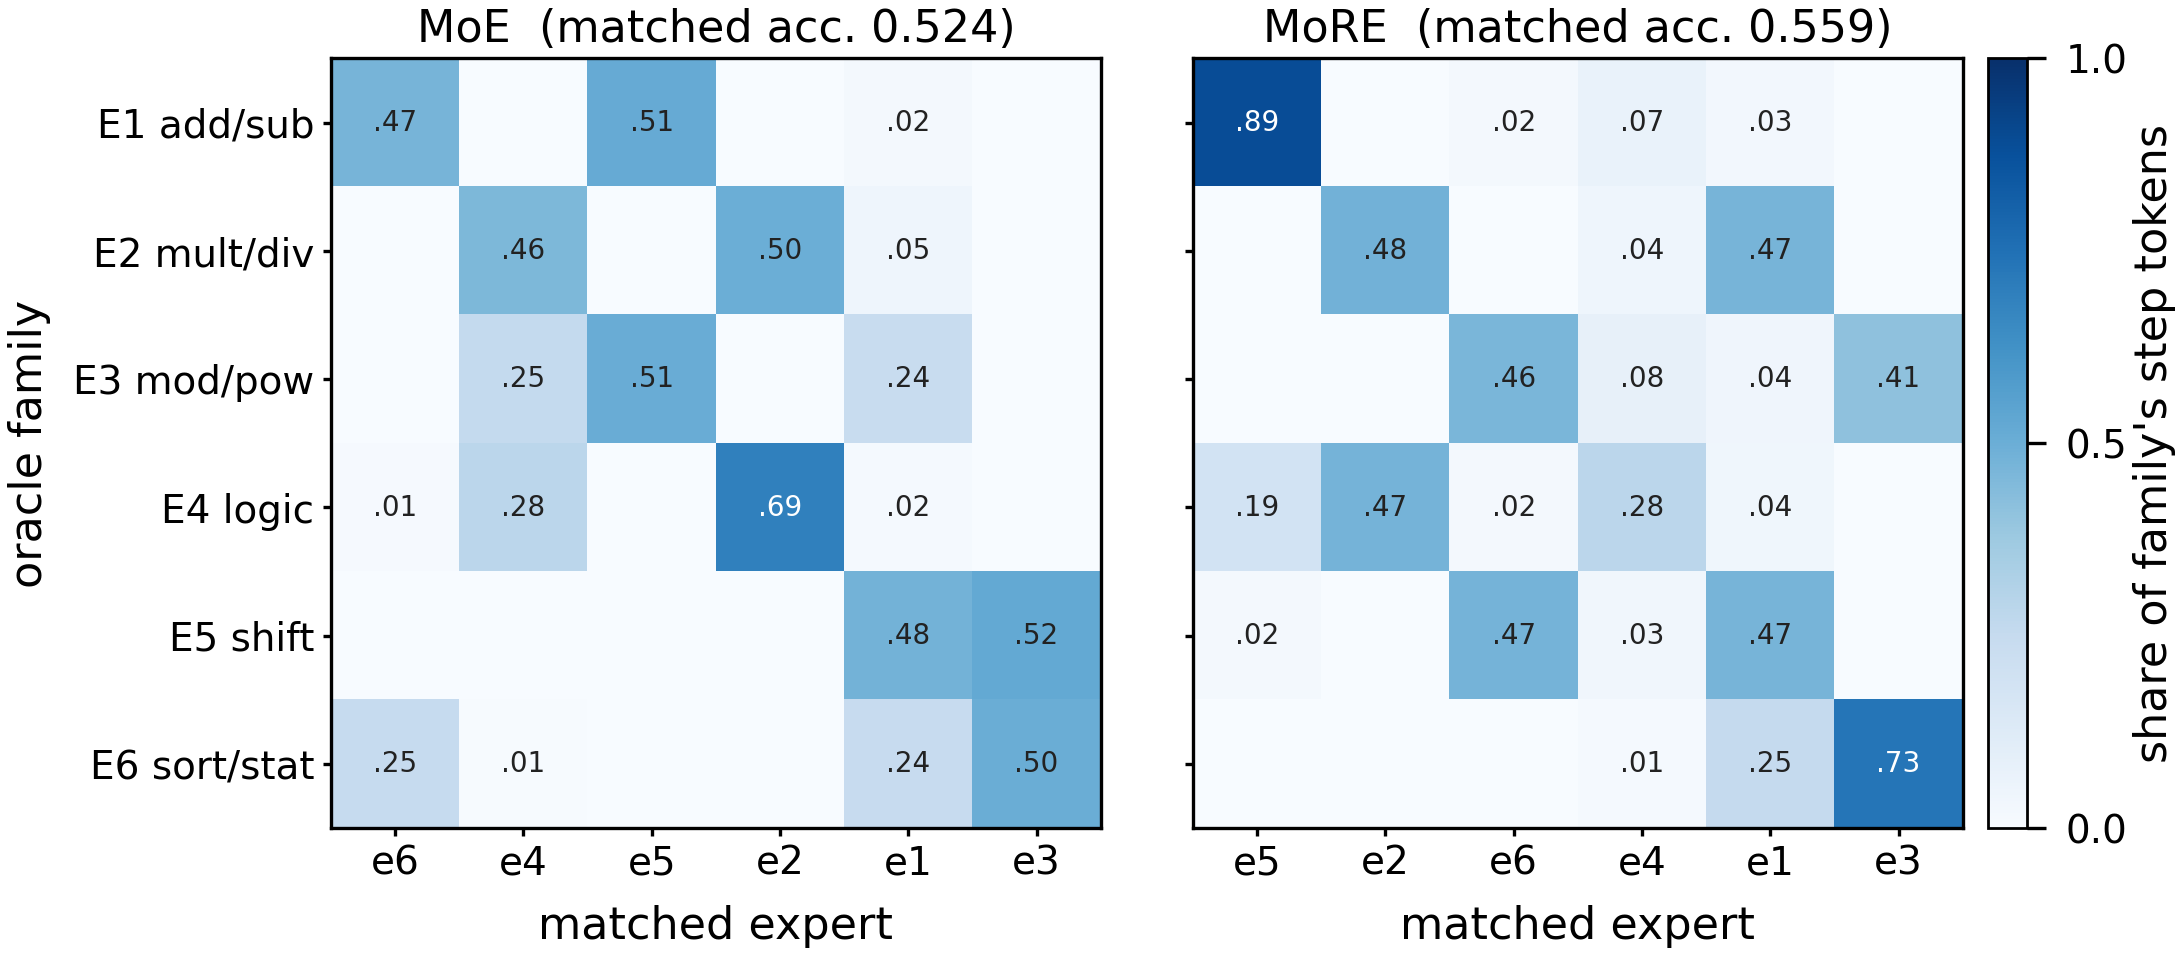
\includegraphics[width=9cm,keepaspectratio]{fig/fig3_routing_confusion.png}
\caption{Routing structure after Hungarian matching, seed 42. Chance is
$1/6 = 0.1667$; the diagonal recovers about half of the oracle partition in
both arms. Columns are matched indices, not learned identities, the
matching is refit per seed, so aggregate values across seeds are reported in
the text rather than averaged into this figure.}
\label{fig:routing}
\end{figure}

\subsection{Ablations}
\label{sec:abl}

Six single-variable variants against the canonical MoRE arm
(Table~\ref{tab:ablations}). Six comparisons on one family of tests means a
Bonferroni-corrected threshold of $\alpha = 0.05/6 = 0.0083$, and we apply it
even where it costs us the more interesting result.

\begin{table}[t]
\centering
\footnotesize
\caption{Ablations against canonical MoRE ($0.063186 \pm 0.000249$). $\Delta$
is validation task loss relative to that arm; positive is worse. $n$ is seeds
completed, which sets the randomization test's floor: $p_{\min} = 0.0040$ at
$n = 5$ and $0.0179$ at $n = 3$, so a 3-seed arm cannot reach the corrected
threshold of $0.0083$ however large its effect. Only rows marked
\textbf{survives} clear that threshold.}
\label{tab:ablations}
\vspace{2pt}
\begin{tabular}{llrrrl}
\toprule
Variant & $n$ & $\Delta$ & $d$ & $p$ & Verdict \\
\midrule
Dense routing (all 6 experts) & 5 & $+0.000529$ & $+1.90$ & 0.0079 & worse, \textbf{survives} \\
Routing supervision on        & 5 & $+0.000565$ & $+2.89$ & 0.0079 & worse, \textbf{survives} \\
Fixed depth $T = 7$           & 5 & $-0.000301$ & $-1.48$ & 0.0476 & better, does \emph{not} survive \\
Ponder weight $\times 0.1$    & 3 & $+0.000444$ &      & 0.1607 & inconclusive ($p_{\min}\,0.0179$) \\
Router noise on               & 3 & $+0.000176$ &      & 0.4107 & inconclusive \\
Two blocks ($+98.6\%$ params) & 3 & $+0.000072$ &      & 0.7500 & inconclusive \\
\bottomrule
\end{tabular}
\end{table}

\textbf{Sparsity earns its place.} Evaluating all six experts and blending them costs $0.000529$ in loss and runs $1.37\times$ faster than Top-1 at six times the expert arithmetic; the gather/scatter, not multiplication, is the overhead for Top-1 (\S\ref{sec:cost}). Dense routing degrades the partition (matched accuracy $0.472$ vs. $0.526$, AMI $0.393$ vs. $0.491$), as expected from removing the pressure to choose.

\textbf{Supervising the router does not help the task.} Adding a cross-entropy term on the oracle expert drives every routing metric to $1.0000 \pm 0.0000$ (perfect matched accuracy, AMI, and purity) but worsens task loss to $0.000565$. Perfect specialization can be forced but is not what the task desires, showing the oracle family partition does not minimize regression loss.

\textbf{Removing adaptivity improves loss, nominally.} Forcing all seven steps per token yields $0.062886 \pm 0.000143$, $0.000301$ better than canonical MoRE at $p=0.0476$. This is below $0.05$ but above the corrected $0.0083$, so it does not survive correction and does not prove adaptive halting harmful. Importantly, the adaptive mechanism does not improve quality: depth allocation error is $5.885$ (expected when all tokens use seven steps), but loss is no worse and throughput ($2198 \pm 274$ toks/s) matches canonical MoRE’s ($2225 \pm 274$) despite $3.4\times$ more steps. Adaptive halting saves arithmetic time not actually spent in this implementation.

\textbf{The three 3-seed arms are inconclusive by design.} At $n=3$, the exact test floors at $p_{\min} = 0.0179$, above the corrected threshold, so none are resolvable. Two remain informative directionally: weakening the ponder penalty $10\times$ raises mean held-out depth from $2.38$ to $2.77$ and worsens depth allocation, so the near-constant policy of \S\ref{sec:depth} is not from an overly strong penalty. Doubling parameters to $6{,}358{,}553$ across two blocks increased loss by $+0.000072$ and reduced throughput $29\%$, consistent with \S\ref{sec:quality}: capacity is not limiting at this scale. Appendix~\ref{app:threeseed} reports details.

\subsection{The cost of conditional computation}
\label{sec:cost}

Throughput distinguishes the three arms far more sharply than loss. MoE trains at $8485 \pm 362$ tokens/s, MoR at $4574 \pm 713$ ($0.54\times$), and MoRE at $2225 \pm 274$ ($0.26\times$, i.e., $3.81\times$ slower than MoE). Arithmetic runs otherwise: counting FFN width-units evaluated, MoRE does $4.75\mathrm{e}8$ vs. MoE's $2.30\mathrm{e}8$ and MoR's $2.77\mathrm{e}9$. MoR performs $5.8\times$ more expert arithmetic than MoRE, yet is still $2.06\times$ faster.

The mechanism causing this is dispatch, not multiplication. Both recursive arms average $2.1$–$2.4$ steps and evaluate exactly one expert per token per step ($1.0000 \pm 0.0000$ evaluations per token, versus $6$ under the dense ablation). Per step, MoRE gathers tokens into six narrow buffers, runs six small matrix multiplications, and scatters results; MoR runs one wide multiplication on a contiguous batch this penalty repeats each recursion step. Two observations support this: the dense ablation evaluates six times the arithmetic and runs $1.37\times$ faster, as it replaces gather/scatter with one blend; and in a batch sweep, a $64\times$ increase in batch size raised wall-clock time by only $2.5\times$, indicating a launch-bound rather than arithmetic-bound workload.

These are end-to-end training throughputs on one consumer GPU, not kernel benchmarks; no claims about cost scaling with model width are made our width sweep failed its consistency check and was rejected (Appendix~\ref{app:cost}).

Practically, it's uncomfortable: MoRE spends $3.81\times$ MoE's wall clock and roughly twice its arithmetic to obtain a loss difference indistinguishable from zero across five seeds, while the fixed-depth variant achieves slightly better loss at the same throughput with fully predictable per-token latency.

\section{Discussion}
\label{sec:discussion}

\subsection{What the measurements support}

Sparse expert routing recovers about half the oracle partition without supervision, maintains load balance, and offsets its dispatch cost versus dense blending, but does not improve task performance. Adaptive halting fails despite functioning mechanically; gradients reach halt heads, tokens exit early, and mean step count matches target, yet behaves near-constantly, with a constant-depth sweep outperforming it on all seeds. Combining a working with a failing mechanism yields worse results.

The key insight is that mean step count and exit histograms, standard adaptive-depth metrics, can be satisfied by input-agnostic policies; both arms meet these yet lack input dependence. Thus, adaptive computation claims require comparison against the best constant budget at the same mean, which demands a held-out data sweep without which halting appears vacuous.

A plausible explanation is the loss design: ponder cost penalizes depth but does not reward matching depth to difficulty; task loss ($R^2 \approx 0.22$) weakly guides this coarse decision. Hence, a near-constant depth is a good solution to the objective but poor for the intended problem.

Contrary to expectations, forcing all tokens to maximum depth yields better loss, identical throughput, and predictable latency. If scalable, adaptive depth introduces undesirable input-dependent latency without throughput gains, making it a poor trade-off for latency-sensitive deployment.

\section{Limitations}\label{sec:limitations}
\label{sec:limits}

Three properties of this study bound what the null result licenses. We state them as bounds on the conclusion, not reasons to discount the measurements: within the regime we ran, the numbers are what they are.

\textbf{Scale.} Each arm has about $3.2$M parameters, $d=256$, one shared block, and was trained on one laptop GPU. Sparse routing is typically argued for when parameter count can grow at roughly constant per-token FLOPs; at matched parameters, that argument does not apply, which is the narrower comparison we sought. The two-block ablation and flat $R^2$ across arms suggest capacity is not limiting here, so the interaction sought may only appear under different conditions.

\textbf{The benchmark.} \texttt{more6-v1} is synthetic: 16 operations grouped into six families by hand, with a hand-authored depth curriculum. Thus, the oracle partition we measure routing against is our design choice; \S\ref{sec:abl} shows the regression objective prefers a different one, and the depth targets encode our belief about operation difficulty, so a model could allocate depth differently and perform poorly on ours. The constant-depth baseline is immune, scored on the same targets, so comparison is internally valid regardless of target meaning.

\textbf{The evaluation.} One scalar regression loss, one fixed split, five seeds, $50$ epochs. Hyperparameters were fixed and validated as stable, not tuned per architecture, so a per-arm search could reorder Table~\ref{tab:main}; the small gaps make this a real risk. The family-classification weight of $0.5$ was inherited rather than selected. We report exact randomization tests and avoid ``statistically significant''; at $n=5$, the smallest attainable $p$ is $0.0040$, and the three $n=3$ arms cannot reach the corrected threshold.

\textbf{Smaller caveats.} Depth statistics come from each run's best-validation checkpoint, while the loss metric is from the final epoch, so they are not from identical weights; depth ablation baselines share the same seed subset as their compared arms; and the dispatch metric \texttt{max\_load\_fraction} reads $1.0$ for recursive arms as an aggregation artifact, not routing collapse. Appendix~\ref{app:caveats} explains each.

\section{Conclusion}
\label{sec:conclusion}

We built the composition of sparse expert routing and adaptive recursion as a
single engine, held parameters and inputs fixed across its three
configurations, and measured what the combination adds. At $3.2$M parameters on
a synthetic arithmetic-reasoning benchmark, it adds nothing: MoRE is
indistinguishable from routing alone in loss, worse than recursion alone,
$3.81\times$ slower than routing alone, and its halting policy is beaten on
every seed by a constant depth chosen by a one-dimensional sweep. Routing
works and does not help; halting is mechanically active and behaviorally
vacuous. We report this as a negative result at this scale and experiment construction rather than a
property of the idea, and we release the engine, the benchmark and the
constant-depth control the last of which we would recommend as a standard
check before any future adaptive-computation model is described as adaptive.

% ===================================================================
% References. Not counted against the 9-page content limit
% (neurips_2026.tex:130-131, :456).
% Build: pdflatex -> bibtex -> pdflatex -> pdflatex
% ===================================================================
\bibliographystyle{plainnat}
\bibliography{refs}

% ===================================================================
% MANDATORY. "The papers not including the checklist will be desk
% rejected." Page-free, like the references. All 16 items are answered
% (9 Yes / 1 No / 6 NA); the instruction block has been deleted per the
% template's own directive while the questions and guidelines are
% verbatim. The justifications name specific sections and specific
% numbers, so if a section is renumbered or a claim changes, re-read
% checklist.tex as part of the rp_rules.md S37 audit. Two answers are
% judgment calls rather than reflex: item 5 (open access) is No because
% no anonymized archive accompanies the submission, and item 10
% (broader impact) is Yes on the strength of app:impact below, which
% exists so that the answer is true.
% ===================================================================
\newpage
\input{checklist}

% ===================================================================
% Appendix. Also page-free (neurips_2026.tex:130-131). Everything here
% was moved OUT of the main body when the estimated page count came in
% over the 9-page ceiling; each block is referenced from the section it
% came from, so nothing was lost, only relocated. If the compiled paper
% turns out to have room, the material can move back -- check
% preflight.py's page estimate before deciding.
% ===================================================================
\newpage
\appendix

\section{Additional experimental detail}
\label{app:detail}

\textbf{Input-contract audit.} An automated audit checks three properties of
the input representation. Mutating a step's stored result changes zero input
features, so the regression target is absent from the input. Permuting the
oracle expert index changes zero input features, so routing cannot be read off
the input. And the feature range is identical at $E \in \{1,5,6\}$, which is
the machine check behind the claim that inputs are bit-identical across arms.
On the normalized target, predicting the training mean gives MSE $0.080914$ and
copying the best single input feature gives $0.081853$. The answer coincides
with one of the step's own arguments for $33.5\%$ of records  an unavoidable
consequence of \textsc{max}, \textsc{min} and \textsc{mod}  but since the
best copy is worse than the constant, the coincidence carries no exploitable
signal. All $R^2$ in the paper are against the $0.080914$ floor.

\textbf{Is specialization label-driven?}
\label{app:famcls}
The canonical objective includes a family-classification term at weight $0.5$
that sees external annotation, so part of the routing structure reported in
\S\ref{sec:routing} may be supervision rather than emergence. We removed that
term entirely in an exploratory configuration at $20$ epochs and $3$ seeds.
This is a proxy setting  neither the canonical epoch count nor the canonical
seed set  so it is not admissible next to Table~\ref{tab:main} and appears
only here. Chance-corrected matched accuracy retained $75.7\%$ of its value
($0.5147 \to 0.4300$), AMI $72.2\%$ ($0.4940 \to 0.3568$) and purity $80.1\%$
($0.5881 \to 0.5041$), with task loss unchanged and no routing collapse. The
structure is therefore not purely label-driven, but the canonical routing
numbers should be read as an upper bound on emergent specialization rather than
a measurement of it.

\textbf{The three underpowered ablation arms.}
\label{app:threeseed}
Three variants completed $3$ of $5$ seeds. At $n = 3$ versus $5$ the exact
randomization test floors at $p_{\min} = 0.0179$, above the
Bonferroni-corrected threshold of $0.0083$, so none of them could have been
resolved however large its effect; we report them as directional evidence only.
Weakening the ponder penalty by $10\times$ raised mean held-out depth from
$2.3810 \pm 0.1379$ to $2.7721 \pm 0.0746$ and raised forced exits to
$0.0104 \pm 0.0089$, while making depth allocation \emph{worse}
($1.1495 \pm 0.0568$ against $1.0282 \pm 0.1320$ on the same three seeds 
note this baseline differs from the five-seed value $0.9940 \pm 0.1054$ in
Table~\ref{tab:depth}, and the two must never be mixed). So the near-constant
policy of \S\ref{sec:depth} is not an artifact of an over-strong depth penalty.
Two blocks raised parameters from $3{,}201{,}555$ to $6{,}358{,}553$
($+98.6\%$), moved loss by $+0.000072$ ($p = 0.7500$) and cost $29\%$ of
throughput ($1587 \pm 187$ tok/s). Router noise moved loss by $+0.000176$
($p = 0.4107$) and cost matched accuracy ($0.4853 \pm 0.0237$ against
$0.5538 \pm 0.0468$ on those seeds).

\textbf{Throughput measurement caveats.}
\label{app:cost}
Roughly $2.4\times$ of measured wall clock sits outside the forward, backward
and optimizer step, so the figures in \S\ref{sec:cost} are end-to-end training
throughputs for this implementation on one RTX 4060 Laptop GPU, not kernel
benchmarks. A fused or grouped expert kernel would change the constants,
although the per-step gather/scatter structure that causes the penalty would
remain. We make no claim about how this cost scales with model width: our width
sweep produced a $d = 512$ configuration that finished faster than $d = 256$
under thermal downclocking, violating its own internal consistency check, and
was rejected as a measurement. No width-versus-cost or width-versus-quality
number appears anywhere in this paper.

\textbf{Caveats attached to specific numbers.}
\label{app:caveats}
Depth statistics are computed offline from each run's best-validation
checkpoint while the primary loss metric is the final epoch, so a depth number
and a loss number are not guaranteed to describe the same weights; the depth
analysis needs one well-defined checkpoint, and the loss metric must avoid an
order-statistic selection effect, and no single choice satisfies both. The
dispatch metric \texttt{max\_load\_fraction} reads $1.0$ for both recursive
arms. This is an aggregation artifact of taking a maximum over recursion steps
whose deep tail is nearly empty, not evidence of routing collapse; normalized
load entropy of $0.99$ is the number to read for balance. Of the runs on disk,
$114$ directories were refused by the results exporter for failing the
canonical-spec match, and only the $5$ admitted seeds per arm feed any table
here.

% Broader impact lives in the appendix rather than the body for page-budget
% reasons: the checklist item is answered \answerYes{} and points here, which
% the checklist instructions permit ("All supporting evidence can appear either
% in the main paper or the supplemental material, provided in appendix").
\textbf{Broader impact.}
\label{app:impact}
This is a small-scale architectural study on synthetic data, so its realistic
effect runs through other researchers' decisions rather than through any
deployment. Conditional computation is pursued because it promises cheaper
inference, and a parameter-matched null result together with a cheap diagnostic
-- score any learned depth policy against the best constant depth before calling
it adaptive -- should save other groups compute on a mechanism that is not
paying for itself. The symmetric risk is that a null obtained at $3.2$M
parameters on hand-authored arithmetic discourages work that would succeed at
scale; \S\ref{sec:limits} scopes the conclusion for exactly that reason. The
models trained here regress a scalar from synthetic arithmetic programs and have
no capability that could be misused.



\end{document}
